\documentclass[10pt,a4paper]{article}
\usepackage[margin=18mm]{geometry}
\usepackage[T1]{fontenc}
\usepackage{lmodern,graphicx,booktabs,hyperref}
\hypersetup{colorlinks=true,urlcolor=blue}
\pagestyle{empty}\setlength{\parindent}{0pt}\setlength{\parskip}{6pt}
\begin{document}
{\LARGE Expanded public-target qualification}\par
23 November 2026. Classical/native/local only; S3 excluded.

\textbf{Observed.} Parent, candidate and C/OpenSSL agree on all 48 public
headers: 12 match archived inputs, and 36 additional targets have been
constructed and admitted. Each of six domains has eight distinct points.
No new cohort solver call has occurred. Unsigned producer observations;
independent reviewer execution and signed standing remain open.
[pcc:unverified]

\begin{minipage}{0.48\linewidth}
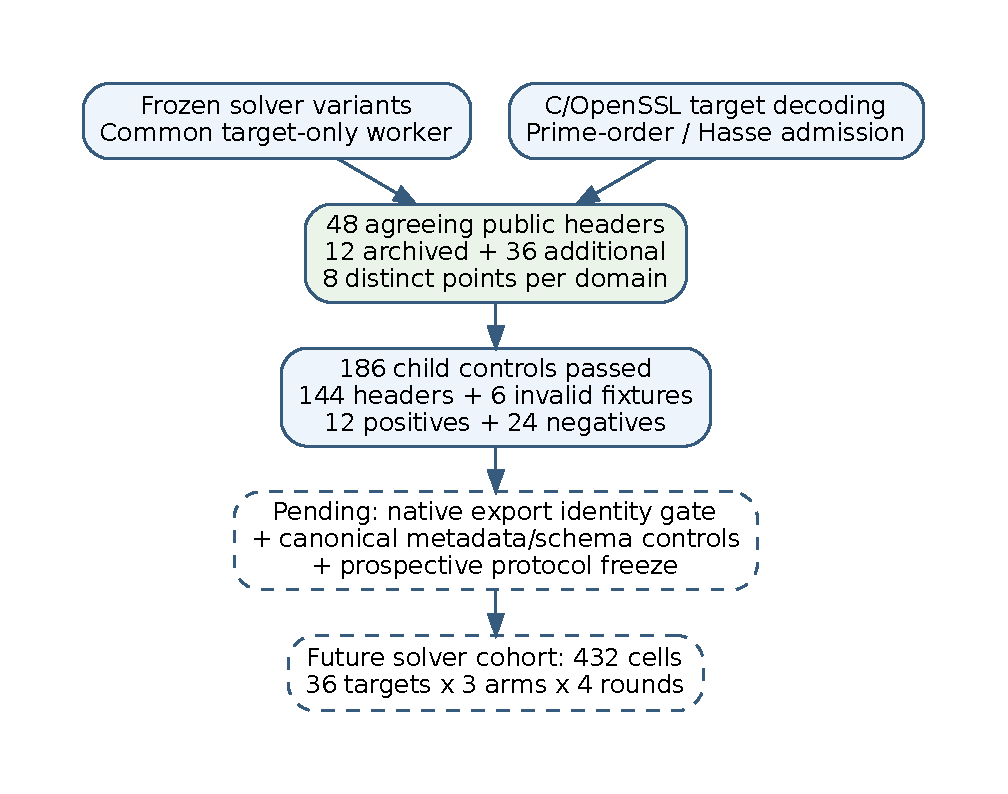
\includegraphics[width=\linewidth,height=76mm,keepaspectratio]{qualification-figure.pdf}
\end{minipage}\hfill
\begin{minipage}{0.49\linewidth}
\begin{tabular}{lr}
\toprule
Copied unit controls & Passed \\
\midrule
Collector / auditor & 11 / 2 \\
Parent / candidate library & 47 / 47 \\
Public-header parser & 4 \\
\midrule
Child census & Passed \\
\midrule
Target-only calls & 144 \\
Invalid fixtures & 6 \\
Old known-answer positives & 12 \\
Wrong scalar / substituted target & 12 / 12 \\
\bottomrule
\end{tabular}
\end{minipage}

\textbf{Isolation.} Both libraries remain byte-identical to their recorded
variants; only a common worker whitelist and target-only branch are new.
The 108-path source copies retain the sole original CPUlib difference.
The C decoder uses Euler/square-root operations and the frozen admission
code. Replay uses raw addition/doubling without a configured group order.
Archived scalars are a separate C-validation input; target-only modes
return before oracle creation or scalar recovery. Seeds 303, 404, 505,
606, 707 and 808 form a deterministic census, not independent uniform
samples. [pcc:unverified]

\textbf{Reproducibility.} Source/input/binary/runtime manifests and raw logs
accompany the source. The 41,576-byte archive extracts without differences
and repacks byte-identically. Build and qualification returned exit 0 with
no sampled memory/disk stop. Rust 1.99.1, locked offline release, one worker;
strict C11/O2. Phase cap 600 s, target child cap 60 s; memory stop
15,032,385,536 bytes, disk launch/stop 256/64 MiB. Cache cleanup retained
copied qualifier hashes. The shell-policy rejection and first Cargo clean's
missing-rustc error are preserved; the pinned-RUSTC retry succeeded.
No scientific census was retried. [pcc:unverified]

\textbf{Next gate.} The canonical checker skips derived seed-table
comparison for \texttt{harness\_drawn}. Its metadata/schema acceptance does
not enforce this fixed named target/seed contract. Complete native export
identity/substitution controls and prospective protocol freeze before
the 432-cell main: 36 targets, 3 arms, one warmup plus three measured
rounds. Main caps stay 1500/120/120 s. Preserve the original 360 calls
and 324 export findings. These phases provide no clock ranking.
[pcc:unverified]

\textbf{Sources and evidence.}
\href{https://github.com/isogeny-labs/crypto/tree/codex/hashed-ecdl-cohort-validation-20261123/research/hashed_ecdl_cohort_validation_20261123/cohort}{Report, source, receipts and archive};
\href{https://www.secg.org/sec1-v2.pdf}{SEC1v2 section 3.1.1.2.1};
\href{https://math.mit.edu/classes/18.783/2025/LectureNotes7.pdf}{Sutherland Lecture 7}.
The full report pins source reconstruction, canonical excerpts and the
prospective plans. KB/Conductor unavailable; no novelty clearance is
inferred. [pcc:unverified]
\end{document}
